\chapter{The Introduction}

This document presents an overview on some security issues that affect the Extensible Authentication Protocol.
This document introduces some basic concepts about EAP, its basic architecture and functionality. It later describes specific security flaws in a implementation of EAP -Subscriber Identity Module SIM. Finally is discusses some enchantments in EAP-SIM to improve the security of these protocols. In this section we discuss the EAP protocol and it's working.
 
\section{Extensible Authentication Protocol Overview} 

The Extensible Authentication Protocol (EAP) is an Internet standard that provides an infrastructure for network access clients and authentication servers. Extensible Authentication Protocol (EAP) enables the dynamic selection of the authentication mechanism at authentication time based on information transmitted in the Access-Request (that is, via RADIUS). Originally, EAP was created as an extension to PPP that allows for the development of arbitrary 
plug-in modules for current and future authentication methods and technologies [3110].Today, EAP is most often used in wireless LANs. Particularly, two wireless standards, WPA and WPA2, which have officially adopted several EAP 
methods as their main authentication mechanisms. 

Lately convergence of Wireless Local Area Networks (WLANs) and 3G systems is currently being deployed from the Third Generation Partnership Project (3GPP), which provides an interworking architecture as an add-on to the 3GPP cellular system specification. The integration of the two systems aims at combining them in such a way that brings out the functional advantages of each technology in a smooth way. The advantages of the cellular technology are related to the roaming capability, the subscription management and the authentication and key agreement procedure. On the other hand, WLANs provide better bandwidth and processing capabilities. To materialize this integration and ensure cooperation at the level of security, the EAP-SIM authentication and session key agreement protocol has been designed for the Global System for Mobile communications (GSM)/General Packet Radio Services (GPRS) network.

\section{EAP- Basics}

EAP was originally created as an extension to PPP to allow for the development of arbitrary network access authentication methods. With EAP, the specific authentication mechanism is not chosen during the link establishment phase of the PPP connection; instead, the PPP peers negotiate to perform EAP during the connection authentication phase. When the connection authentication phase is reached, the peers negotiate the use of a specific EAP authentication scheme known as an EAP method. After the EAP method is agreed upon, EAP allows for an open-ended exchange of messages between the access client and the authenticating server that can vary based on the parameters of the connection. The conversation consists of requests and responses for authentication information. The EAP method determines the length and details of the authentication conversation. Architecturally, an EAP infrastructure consists of the following:
EAP peer Computer that is attempting to access a network, also known as an access client. EAP authenticator An access point or network access server (NAS) that is requiring EAP authentication prior to granting access to a network. Authentication server A server computer that negotiates the use of a specific EAP method with an EAP peer, validates the EAP peer's credentials, and authorizes access to the network. Typically, the authentication server is a Remote Authentication Dial-In User Service (RADIUS) server. EAP is extensible through EAP methods that plug-in at both the EAP peer and authenticating server ends of a connection. To add support for a new EAP method, you install an EAP method library file on both the EAP peer and the authenticating server. This capability to extend EAP provides vendors with the opportunity to create new authentication schemes. EAP provides the highest flexibility to allow for more secure authentication methods. The EAP peer and the EAP authenticator send EAP messages using a supplicant-a software component that uses EAP to authenticate network access-and a data link layer transport protocol such as PPP or IEEE 802.1X. The EAP authenticator and the authentication server send EAP messages using RADIUS. The end result is that EAP messages are exchanged between the EAP components on the EAP peer and the authentication server. The following figure shows EAP infrastructure and information flow.

\begin{figure}[htb]
\centering	
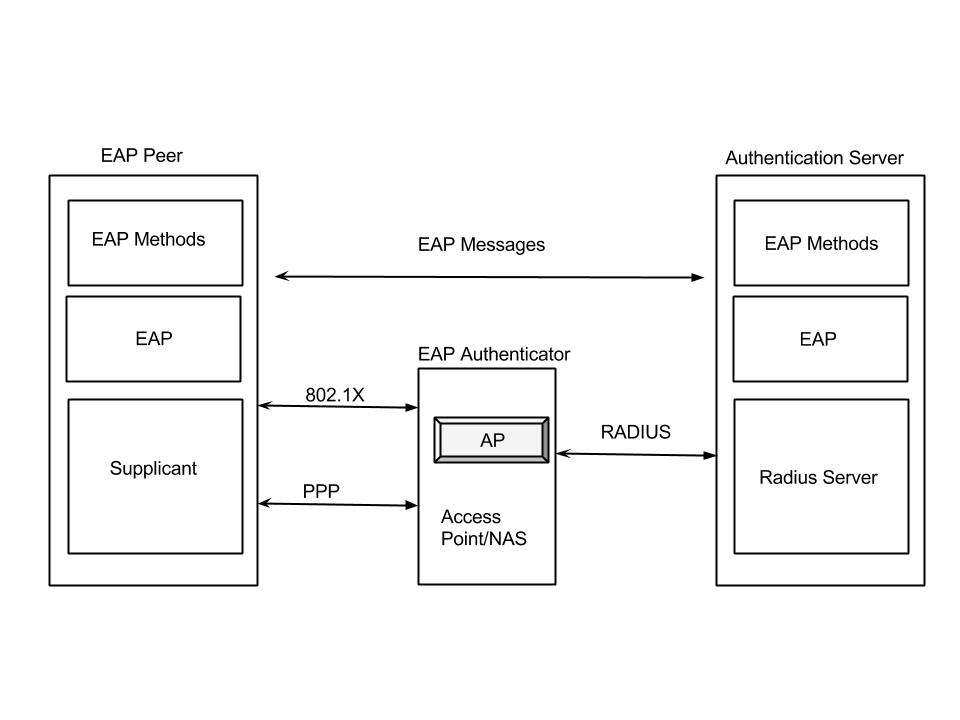
\includegraphics[width=1\textwidth]{images/EAP_overview.jpg}
\caption{EAP Authentication Stack} 
\label{fig:EAP Authentication Stack}
\end{figure}

The main components of EAP, as shown in Figure 1, are the following:
--EAP peer/Access Clients: Computers attempting to access network resources.

--EAP authenticator: An access point (AP) or network access server (NAS) requiring EAP authentication before granting access to a network resource.

--Authentication server: A server computer that negotiates the use of a specific EAP method with an EAP Access Client. It also validates EAP peers’ credentials and authorizes access to network resources. In Figure 1, the authentication server is a Remote Authentication Dial-In User Service (RADIUS) server. Notice from Figure 1 that the EAP peer and, in the case of wireless LANs, the EAP authenticator both send EAP messages using a supplicant and a data link layer transport protocol such as PPP—or, for wireless LANs, the IEEE 802.1X infrastructure. A supplicant is a software component that uses EAP to authenticate network access but that handles the actual data exchange. In the example shown in Figure 1, both the EAP authenticator and the authentication server send EAP messages using
RADIUS. 

As a result, EAP messages are actually exchanged between the EAP components on the EAP client and the authentication server. In a word, EAP provides the highest flexibility because it allows vendors to create more secure authentication schemes that can be plugged in later on, as required.

\section{The EAP protocol family}

EAP is an authentication framework providing for the transport and usage of keying material and parameters generated by EAP methods.[x] There are many methods defined by RFCs and a number of vendor specific methods and new proposals exist. EAP is not a wire protocol; instead it only defines message formats. Each protocol that uses EAP defines a way to encapsulate EAP messages within that protocol's messages. EAP is in wide use. For example, in IEEE 802.11 (WiFi) the WPA and WPA2 standards have adopted IEEE 802.1X with one-hundred EAP types as the official authentication mechanisms.

Most common EAP methods are EAP-MD5, EAP-POTP, EAP-GTC, EAP-TLS, EAP-IKEv2, EAP-SIM, EAP-AKA and EAP-AKA'. Additionally a number of vendor-specific methods and new proposals exist. The figure below describes the basic types on EAP methods. 

\begin{figure}[htb]
\centering	
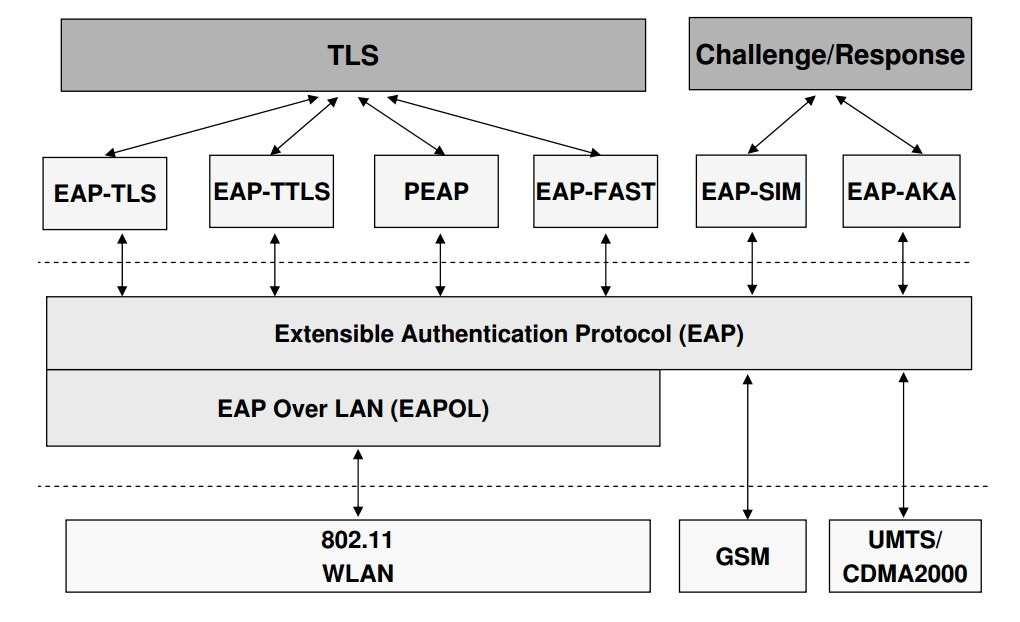
\includegraphics[width=1\textwidth]{images/eap_protocol_family.jpg}
\caption{EAP Protocol Family} 
\label{fig:EAP Protocol Family}
\end{figure}

In Figure 2 we see that EAP protocols EAP-TLS,EAP-TTLS,EAP-FAST,PEAP are based on Transport Layer Security(TLS).  TLS is the successor to the Secure Sockets Layer (SSL).TLS is a protocol that ensures privacy between communicating applications and their users on the Internet. When a server and client communicate, TLS ensures that no third party may eavesdrop or tamper with any message. The EAP TLS based protocols are mainly used for Wireless-LAN. The WPA wireless authentication protocol family is based on EAP TLS protocols. 

EAP-SIM and EAP-AKA are based on Challenge-Response protocol. These protocols are popular among mobile users today. And the special Challenge-Response design on these protocols leads to major security flaws which we will discuss in section II. 